\renewcommand{\thesection}{\Roman{section}}
\titleformat{\section}
{\normalfont\bfseries}{PHẦN~\thesection.}{0.4em}{}
\newcolumntype{C}[1]{>{\centering\arraybackslash}p{#1}}
\newcolumntype{L}[1]{>{\raggedright\arraybackslash}p{#1}}
\begin{tabular}{C{5cm}C{11cm}}
	\textbf{TRUNG TÂM MANABIE}& \textbf{ĐỀ ÔN TẬP KIỂM TRA GIỮA HỌC KÌ 2} \\
	\textbf{ĐỀ 04}& \textbf{Môn: VẬT LÝ}\\
	\textit{(Đề có 04 trang)}& \textit{Thời gian làm bài: 50 phút, không kể thời gian phát đề}
	
	\noindent\rule{4cm}{0.8pt} \\
\end{tabular}
\section{TRẮC NGHIỆM \textit{(6,0 điểm)}}
\ANSMCQ{
	\begin{tabular}{|C{1.2cm}|C{1.2cm}|C{1.2cm}|C{1.2cm}|C{1.2cm}|C{1.2cm}|C{1.2cm}|C{1.2cm}|C{1.2cm}|C{1.2cm}|}
		\hline
		1. A & 2. C & 3. B & 4. B & 5. B & 6. C & 7.D & 8. B & 9. D & 10. D\\
		\hline
		11. C & 12. B & 13. A & 14. A & 15. D & 16. B & 17.B & 18. C & 19. D & 20. C\\
		\hline
		21. C & 22. A & 23. D & 24. D & &  & &  &  & \\
		\hline
	\end{tabular}
}

\begin{enumerate}[label=\bfseries Câu \arabic*:]
	\item Nếu độ lớn điện tích của một trong hai vật nhỏ mang điện tăng gấp đôi, đồng thời khoảng cách giữa chúng tăng lên gấp đôi thì lực tương tác điện giữa hai vật sẽ
	\begin{mcq}(4)
		\item giảm 2 lần.
		\item giảm 4 lần.
		\item tăng 2 lần.
		\item không đổi
	\end{mcq}
\hideall{
\textbf{Đáp án A.}\\
Ta có:
$$\begin{cases}
	F=\dfrac{k\left|q_1q_2\right|}{\varepsilon r^2}\\
	F'=\dfrac{k\left|2q_1q_2\right|}{\varepsilon\left(2r\right)^2}=\dfrac{k\left|q_1q_2\right|}{2\varepsilon r^2}=\dfrac{F}{2}
\end{cases}$$
}

\item Nếu đổi dấu cả hai điện tích điểm nhưng vẫn giữ nguyên độ lớn và vị trí của chúng thì lực tương tác điện giữa hai điện tích sẽ 
\begin{mcq}(4)
	\item thay đổi độ lớn.
	\item thay đổi phương.	
	\item không thay đổi.
	\item điểm đặt.
\end{mcq}
\hideall{
\textbf{Đáp án C.}
}

\item Đưa một quả cầu mang điện tích dương lại gần (không tiếp xúc) đầu A của một thanh trụ sắt AB trung hòa về điện. Chạm tay vào đầu B của thanh sắt rồi bỏ tay ra thì thanh sắt bị nhiễm điện. Chọn phát biểu \textbf{đúng}.
\begin{mcq}
	\item Thanh sắt nhiễm điện dương.
	\item Thanh sắt nhiễm điện âm.
	\item Tổng điện tích của thanh sắt bằng 0.
	\item Tổng điện tích của thanh sắt bằng 0.
\end{mcq}
\hideall{
\textbf{Đáp án B.}
}



\item Cho 2 điện tích điểm có độ lớn không đổi, đặt cách nhau một khoảng không đổi. Lực tương tác giữa chúng sẽ lớn nhất khi chúng đặt trong
\begin{mcq}(2)
	\item nước nguyên chất.
	\item chân không.
	\item dầu hoả.
	\item không khí ở điều kiện tiêu chuẩn.
\end{mcq}
\hideall{
\textbf{Đáp án B.}\\
$$F=\dfrac{k\left|q_1q_2\right|}{\varepsilon r^2}$$
với $\varepsilon\ge 1$ nên $F_\text{max}\Leftrightarrow \varepsilon =1$.
}

\item Hai điện tích điểm đặt cách nhau một khoảng $\SI{30}{\centi\meter}$ trong không khí, lực tương tác giữa chúng là $F$. Nếu đặt chúng trong dầu thì lực này yếu đi 2,25 lần. Để lực tương tác giữa chúng vẫn là $F$ thì cần dịch chuyển chúng một khoảng là
\begin{mcq}(2)
	\item $\SI{0.1}{\centi\meter}$.
	\item $\SI{10}{\centi\meter}$.
	\item $\SI{1}{\centi\meter}$.
	\item $\SI{24}{\centi\meter}$ hoặc $\SI{20}{\centi\meter}$.
\end{mcq}
\hideall{
\textbf{Đáp án B.}\\
$$F'=F\Leftrightarrow \varepsilon r'^2=r^2\Rightarrow r'=\SI{20}{\centi\meter}.$$
}

\item Một quả cầu kim loại mang điện tích $\SI{-7.2E-16}{\coulomb}$. Quả cầu này
\begin{mcq}(2)
	\item thiếu 6240 electron.
	\item thừa 6240 electron.
	\item thừa 4500 electron.
	\item thiếu 4500 electron.
\end{mcq}
\hideall{
\textbf{Đáp án C.}\\
Qủa cầu tích điện âm nên nó thừa electron.\\
Số electron thừa:
$$N=\dfrac{q}{e}=\SI{4500}{\text{
electron}}.$$
}

\item Tổng số proton và electron của một nguyên tử trung hoà có thể là số nào sau đây?
\begin{mcq}(4)
	\item 11.
	\item 13.
	\item 17.
	\item 14.
\end{mcq}
\hideall{
\textbf{Đáp án D.}\\
Vì nguyên tử trung hoà nên số proton bằng số electron $\Rightarrow$ tổng số proton và electron phải là số chẵn.
}

\item Độ lớn cường độ điện trường tại một điểm gây bởi một điện tích điểm \textbf{không phụ thuộc} vào
\begin{mcq}(2)
	\item độ lớn điện tích đó.
	\item độ lớn điện tích thử.
	\item khoảng cách từ điểm đang xét đến điện tích đó.
	\item hằng số điện môi của môi trường.
\end{mcq}
\hideall{
\textbf{Đáp án B.}\\
Độ lớn cường độ điện trường tại một điểm gây bởi một điện tích điểm không phụ thuộc vào độ lớn của điện tích thử.
}

\item Khi một electron chuyển động ngược hướng với vectơ cường độ điện trường thì
\begin{mcq}(2)
	\item thế năng của nó tăng, điện thế của nó giảm.
	\item thế năng và điện thế đều tăng.
	\item thế năng và điện thế đều giảm.
	\item thế năng giảm, điện thế tăng.
\end{mcq}
\hideall{
\textbf{Đáp án D.}\\
Khi một electron chuyển động ngược hướng với vectơ cường độ điện trường thì điện thế tăng (vector cường độ điện trường hướng từ nơi có điện thế cao về nơi có điện thế thấp).\\
Ta có:
$$W_{t_M}-W_{t_N}=e\left(V_M-V_N\right)>0 \Rightarrow W_{t_M}>W_{t_N}$$
Như vậy trong quá trình dịch chuyển thì thế năng giảm.
}

\item Phát biểu nào sau đây \textbf{không đúng} khi nói về đường sức điện?
\begin{mcq}
	\item Tại mỗi điểm trong điện trường ta chỉ vẽ một đường sức đi qua. 
	\item Các đường sức là những đường cong không kín.
	\item Các đường sức không bao giờ cắt nhau. 
	\item Các đường sức điện luôn xuất phát từ điện tích dương và kết thúc ở điện tích âm.
\end{mcq}
\hideall{
\textbf{Đáp án D.}}

\item Công của lực điện tác dụng lên một điện tích điểm q khi di chuyển từ điểm M đến điểm N trong điện trường, thì \textbf{không phụ thuộc} vào
\begin{mcq}(2)
	\item độ lớn của điện tích $q$.
	\item vị trí của điểm M và N.
	\item hình dạng của đường đi MN.
	\item độ lớn của cường độ điện trường.
\end{mcq}
\hideall{
\textbf{Đáp án C.}\\
Công lực điện không phụ thuộc vào hình dạng đường đi.
}

\item Điện thế là đại lượng đặc trưng riêng cho điện trường về
\begin{mcq}
	\item  khả năng sinh công của vùng không gian có điện trường.
	\item khả năng sinh công khi đặt tại đó một điện tích. 
	\item khả năng tác dụng lực tại một điểm.
	\item khả năng tác dụng lực tại tất cả các điểm trong không gian có điện trường.
\end{mcq}
\hideall{
\textbf{Đáp án B.}\\
Ý nghĩa vật lý của điện thế là đặc trưng cho khả năng sinh công của điện trường khi đặt tại đó một điện tích.
}

\item Điện tích điểm $q=\SI{10}{\micro\coulomb}$ chuyển động từ đỉnh B đến đỉnh C của tam giác đều ABC cạnh $\SI{10}{\centi\meter}$, nằm trong điện trường đều, cường độ $\SI{5000}{\volt/\meter}$, đường sức song song với BC và có chiều từ C đến B. Công của lực điện khi điện tích chuyển động theo đoạn thẳng BC và theo đoạn gấp khúc BAC là
\begin{mcq}
	\item $A_\text{BC}=\SI{-5E-3}{\joule}$, $A_\text{BAC}=\SI{-5E-3}{\joule}$.
	\item $A_\text{BC}=\SI{-2.5E-4}{\joule}$, $A_\text{BAC}=\SI{-2.5E-4}{\joule}$.
	\item $A_\text{BC}=\SI{-2.5E-4}{\joule}$, $A_\text{BAC}=\SI{-5E-4}{\joule}$.
	\item $A_\text{BC}=\SI{-5E-4}{\joule}$, $A_\text{BAC}=\SI{E-4}{\joule}$.
\end{mcq}
\hideall{
\textbf{Đáp án A.}\\
$$A_\text{BC}=A_\text{BAC}=qE\cdot BC\cos\SI{180}{\degree}=\SI{-5E-3}{\joule}.$$
}

\item Hiệu điện thế giữa hai điểm   là M và N là $U_\text{MN}=\SI{30}{\volt}$. Điện thế tại N là $\SI{10}{\volt}$. Điện thế tại M là 
\begin{mcq}(4)
	\item $\SI{40}{\volt}$.
	\item $\SI{20}{\volt}$.
	\item $\SI{-40}{\volt}$.
	\item $\SI{-20}{\volt}$.
\end{mcq}
\hideall{
\textbf{Đáp án A.}\\
$$U_\text{MN}=V_\text{M}-V_\text{N}\Rightarrow V_\text{M}=\SI{40}{\volt}.$$
}

\item Hai tấm kim loại phẳng, nằm ngang song song, cách nhau $d=\SI{5}{\centi\meter}$. Cường độ điện trường giữa hai bản là $\SI{E4}{\volt/\meter}$. Điện thế tại M các bản dương $\SI{2}{\centi\meter}$ là 
\begin{mcq}(4)
	\item $\SI{200}{\volt}$.
	\item $\SI{500}{\volt}$.
	\item $\SI{700}{\volt}$.
	\item $\SI{300}{\volt}$.
\end{mcq}
\hideall{
\textbf{Đáp án D.}\\
$$V_\text{M}-V_-=E\cdot d_{M-}\cos\SI{0}{\degree}=\left(\SI{E4}{\volt/\meter}\right)\cdot\left(\SI{3E-2}{\meter}\right)=\SI{300}{\volt} \Rightarrow V_\text{M}=\SI{300}{\volt}.$$
}

\item Một quả cầu nhỏ khối lượng $m=\SI{50}{\gram}$ mang điện tích $q=\SI{-5E-6}{\coulomb}$ được treo bằng một dây mảnh, không dãn, không dẫn điện. Hệ trên được đặt trong trọng trường đều $\vec{g}$ và điện trường đều $\vec{E}$ có phương thẳng đứng. Lấy $g=\SI{10}{\meter/\second^2}$. Khi quả cầu cân bằng, dây treo không bị căng. Độ lớn $E$ của cường độ điện trường đều là
\begin{mcq}(4)
	\item $\SI{E4}{\volt/\meter}$.
	\item $\SI{E5}{\volt/\meter}$.
	\item $\SI{E6}{\volt/\meter}$.
	\item $\SI{5E4}{\volt/\meter}$.
\end{mcq}
\hideall{
\textbf{Đáp án B.}\\
Vì khi quả cầu cân bằng, dây không căng nên:
$$P=F_\text{đ}\Leftrightarrow mg=\left|q\right|E$$
$$\Rightarrow E=\dfrac{mg}{\left|q\right|}=\SI{E5}{\volt/\meter}.$$
}

\item Cho hai quả cầu kim loại bán kính bằng nhau, tích điện cùng dấu tiếp xúc với nhau. Các điện tích phân bố như thế nào trên hai quả cầu đó nếu một trong hai quả cầu là rỗng?
\begin{mcq}
	\item Quả cầu đặc phân bố đều trong cả thể tích, quả cầu rỗng chỉ ở mặt ngoài.
	\item Quả cầu đặc và quả cầu rỗng chỉ phân bố ở mặt ngoài.
	\item Quả cầu đặc và quả cầu rỗng phân bố đều trong cả thể tích. 
	\item Quả cầu đặc phân bố ở mặt ngoài, quả cầu rỗng phân bố đều trong thể tích.
\end{mcq}
\hideall{
\textbf{Đáp án B.}\\
Vật dẫn phân bố điện tích trên mặt ngoài.
}

\item Nối hai bản tụ điện phẳng với hai cực của nguồn một chiều, sau đó ngắt tụ ra khỏi nguồn rồi đưa vào giữa hai bản một chất điện môi có hằng số điện môi $\varepsilon$  thì điện dung $C$  và hiệu điện thế giữa hai bản tụ sẽ
\begin{mcq}(2)
	\item $C$ tăng và $U$ tăng.
	\item $C$ giảm và $U$ giảm.
	\item $C$ tăng và $U$ giảm.
	\item $C$ giảm và $U$ tăng.
\end{mcq}
\hideall{
\textbf{Đáp án C.}\\
Điện dung của tụ điện phẳng:
$$C=\dfrac{\varepsilon S}{4\pi kd }$$
nên điện dung của tụ sẽ tăng khi đưa vào giữa hai bản một chất điện môi. Ngắt tụ khỏi nguồn nên $Q$ không đổi $\Rightarrow U=\dfrac{Q}{C}$ giảm.
}

\item Hai điện tích điểm có độ lớn bằng nhau nhưng trái dấu, đặt cố định tại 2 điểm M và N trong chân không. Vị trí đặt điện tích điểm thứ ba để nó nằm cân bằng là
\begin{mcq}(2)
	\item giữa hai điểm M và N.
	\item trên tia đối của tia MN.
	\item trên tia đối của tia NM.
	\item không tồn tại vị trí nào thỏa mãn.
\end{mcq}
\hideall{
\textbf{Đáp án D.}\\
Vì hai điện tích trái dấu nên vị trí để điện tích thứ 3 cân bằng phải nằm trên đường nối hai điện tích và nằm ngoài hai điện tích.\\
$$F_{1q}=F_{2q}$$
$$\Leftrightarrow \dfrac{k\left|q_1q\right|}{r^2_{1q}}=\dfrac{k\left|q_2q\right|}{r^2_{2q}}$$
Vì $q_1=q_2$ nên $r_{1q}=r_{2q}$. Không có điểm nào thoả mãn điều kiện trên.
}

\item Ba tụ điện có điện dung $C_1=C_2=\dfrac{C_3}{2}=C$. Để được bộ tụ có điện dung là $C$ thì các tụ phải ghép
\begin{mcq}(2)
	\item 3 tụ nối tiếp nhau.
	\item 3 tụ song song nhau.
	\item $\left(C_1//C_2\right)$ nt $C_3$.
	\item $\left(C_1\ \textit{nt}\  C_2\right)$ // $C_3$.
\end{mcq}
\hideall{
\textbf{Đáp án C.}\\
Khi $C_1//C_2 \Rightarrow C_{12}=2C$.\\
Khi $C_{12}$ nt $C_3$ và $C_{12}=C_3=2C\Rightarrow C_b=\dfrac{2C}{2}=C.$
}

\item Một bộ tụ điện gồm 10 tụ điện giống nhau $\left(C=\SI{8}{\micro\farad}\right)$ ghép nối tiếp với nhau. Bộ tụ điện được nối với hiệu điện thế không đổi $U=\SI{150}{\volt}$. Độ biến thiên năng lượng của bộ tụ điện sau khi có một tụ điện bị đánh thủng là
\begin{mcq}(4)
	\item $\SI{9}{\milli\joule}$.
	\item $\SI{10}{\milli\joule}$.
	\item $\SI{1}{\milli\joule}$.
	\item $\SI{19}{\milli\joule}$.
\end{mcq}
\hideall{
\textbf{Đáp án C.}\\
Năng lượng của bộ tụ ban đầu 
$$W_{10C}=\dfrac{1}{2}U^2\left(\dfrac{C}{10}\right).$$
Năng lượng của bộ tụ lúc sau:
$$W_{9C}=\dfrac{1}{2}U^2\left(\dfrac{C}{9}\right).$$
Độ biến thiên năng lượng của bộ tụ điện
$$\Delta W=W_{9C}-W_{10C}=\dfrac{1}{2}U^2\left(\dfrac{C}{9}-\dfrac{C}{10}\right)=\SI{1}{\milli\joule}.$$
}

\item Năng lượng điện trường trong tụ điện tỉ lệ với
\begin{mcq}
	\item bình phương điện tích trên tụ điện.
	\item hiệu điện thế giữa hai bản tụ điện.
	\item điện tích trên tụ điện.	
	\item hiệu điện thế hai bản tụ và điện tích trên tụ.
\end{mcq}
\hideall{
\textbf{Đáp án A.}\\
$$W=\dfrac{1}{2}QU=\dfrac{1}{2}CU^2=\dfrac{Q^2}{2C}$$
$C$ không đổi nên $W\sim Q^2$.
}

\item Công của lực điện trường dịch chuyển một điện tích $\SI{-2}{\micro\coulomb}$ từ A đến B là $\SI{4}{\milli\joule}$. Hiệu điện thế giữa hai điểm A và B có giá trị bằng
\begin{mcq}(4)
	\item $\SI{-8}{\volt}$.
	\item $\SI{2}{\volt}$.
	\item $\SI{2000}{\volt}$.
	\item $\SI{-2000}{\volt}$.
\end{mcq}
\hideall{
\textbf{Đáp án D.}\\
$$U_\text{AB}=\dfrac{A_\text{AB}}{q}=\SI{-2000}{\volt}.$$


}

\item Một tụ điện có điện dung $C$ được tích điện với điện áp $U$. Ngắt tụ khỏi nguồn, giảm điện dung xuống còn một nửa thì năng lượng của tụ
\begin{mcq}(2)
	\item không đổi.
	\item giảm còn một phần tư.
	\item giảm còn một nửa.
	\item tăng gấp đôi.
\end{mcq}
\hideall{
\textbf{Đáp án D.}\\
Điện tích của tụ khi ngắt ra khỏi nguồn sẽ không thay đổi.\\
$$W'=\dfrac{Q^2}{2C'}=\dfrac{Q^2}{2\dfrac{C}{2}}=2W.$$
}
\end{enumerate}
\section{TỰ LUẬN \textit{(4,0 điểm)}}
\begin{enumerate}[label=\bfseries Câu \arabic*:]
	\item \textit{(1,0 điểm)} Khi sửa chữa các thiết bị điện gia dụng có chứa tụ điện, có một quy tắc an toàn mà người sửa điện cần lưu ý đó là không được chạm tay trực tiếp vào 2 chân của tụ điện khi mới tháo khỏi mạch điện. Người sửa điện nên cầm phần thân của tụ và chạm đầu tua vít (có tay cầm cách điện) vào 2 chân tụ đến khi không còn nghe tiếng nổ lách tách hoặc nối hai chân tụ với bóng đèn. Em hãy cho biết vì sao cần phải làm như vậy?
	\begin{center}
		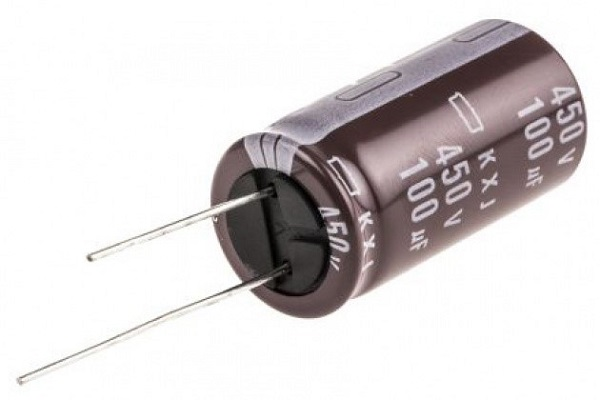
\includegraphics[width=0.25\linewidth]{../figs/PH11-MidSem2-04-1}
		\captionof{figure}{Tụ hoá thường được dùng trong các tivi.}
	\end{center}
	\hideall{
	Tụ điện tích trữ năng lượng dưới dạng năng lượng điện trường khi được nối với nguồn. Mặc dù đã ngắt khỏi nguồn nhưng trong tụ vẫn còn tồn trữ năng lượng. Khi chạm tay trực tiếp vào 2 chân tụ, tụ phóng điện và gây điện giật. Do đó, người sửa điện cần có thao tác xả điện cho tụ. 
}

\item \textit{(2,0 điểm)} Một hạt bụi tích điện âm và có khối lượng $\SI{E-10}{\kilogram}$ nằm lơ lửng chính giữa hai bản tụ điện phẳng nằm ngang. Hiệu điện thế giữa hai bản là $\SI{1000}{\volt}$, khoảng cách giữa hai bản là $\SI{6.4}{\milli\meter}$. Lấy $g=\SI{10}{\meter/\second^2}$.
\begin{enumerate}[label=\alph*)]
	\item Tính cường độ điện trường giữa hai bản tụ điện.
	\item Chiếu tia tử ngoại làm hạt bụi mất đi một số electron thì thấy nó rơi xuống với gia tốc $\SI{4}{\meter/\second^2}$. Tính số electron mà hạt bụi đã mất và tốc độ của hạt bụi khi chạm bản âm
\end{enumerate}
\hideall{
\begin{enumerate}[label=\alph*)]
	\item Cường độ điện trường giữa hai bản tụ điện:
	$$E=\dfrac{U}{d}=\SI{156250}{\volt/\meter}.$$
	\item Hạt bụi nằm lơ lửng nên lực điện cân bằng với trọng lực
	$$\left|q\right|E=mg\Rightarrow q=-\dfrac{mg}{E}=\SI{-6.4E-15}{\coulomb}.$$
	Gọi $q'$ là điện tích của hạt bụi sau khi chiếu tia tử ngoại.\\ 
	Áp dụng định luật II Newton:
	$$mg-\left|q'\right|E=ma\Rightarrow q'=-\dfrac{mg-ma}{E}=\SI{-3.84E-15}{\coulomb}$$
	Số electron đã mất:
	$$N=\dfrac{q'-q}{e}=\SI{16000}{\text{electron}}.$$
	Tốc độ của electron khi chạm vào bản âm
	$$v=\sqrt{2a\dfrac{d}{2}}=\SI{0.16}{\meter/\second}.$$
\end{enumerate}
}

\item \textit{(1,0 điểm)} Tại ba đỉnh của một tam giác vuông OAB (vuông tại O, các cạnh có chiều dài $\SI{10}{\centi\meter}$, $\SI{8}{\centi\meter}$, $\SI{6}{\centi\meter}$), người ta đặt lần lượt các điện tích $q_1, q_2, q_3$ (với $q_1=q_2=q_3=\SI{10}{\pico\farad}$). Gọi H là chân đường cao kẻ từ O của tam giác OAB. Tính độ lớn cường độ điện trường do 3 điện tích gây ra tại H.
\hideall{
\begin{center}
	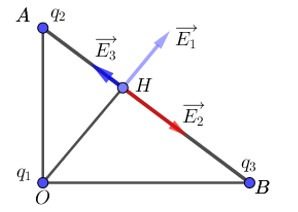
\includegraphics[width=0.3\linewidth]{../figs/PH11-MidSem2-04-2}
\end{center}
Ta có:
\begin{eqnarray*}
	\dfrac{1}{\text{OH}^2}&=&\dfrac{1}{\text{OA}^2}+\dfrac{1}{\text{OB}^2}\Rightarrow \text{OH}=\SI{4.8}{\centi\meter}\\
	\text{AH}&=&\sqrt{\text{OA}^2-\text{OH}^2}=\SI{3.6}{\centi\meter}\\
	\text{BH}&=&\sqrt{\text{OB}^2-\text{OH}^2}=\SI{6.4}{\centi\meter}.
\end{eqnarray*}
Độ lớn cường độ điện trường do các điện tích điểm gây ra tại H:
\begin{eqnarray*}
	E_1&=& \dfrac{k\left|q_1\right|}{\text{OH}^2}=\SI{39.06}{\volt/\meter}\\
	E_2&=&\dfrac{k\left|q_2\right|}{\text{AH}^2}=\SI{69.44}{\volt/\meter}\\
	E_3&=&\dfrac{k\left|q_3\right|}{\text{BH}^2}=\SI{21.97}{\volt/\meter}
\end{eqnarray*}
Cường độ điện trường tổng hợp tại H
$$\vec{E}_\text{H}=\vec{E}_1+\vec{E}_2+\vec{E}_3=\vec{E}_1+\vec{E}_{23}$$
Do $\vec{E}_{23}\bot\vec{E}_1$ nên $E_\text{H}=\sqrt{E^2_1+E^2_{23}}=\sqrt{E^2_1+\left(E_2-E_3\right)^2}\approx\SI{61.47}{\volt/\meter}.$
}
\end{enumerate}
\begin{center}
	\textbf{--- HẾT ---}
\end{center}
